\documentclass[a4paper]{article}
\usepackage[spanish,es-lcroman]{babel}
\usepackage[utf8]{inputenc}
\spanishdecimal{.}
\usepackage{bm}
\usepackage{amssymb}
\usepackage{mathtools}
\usepackage{amsmath}
\usepackage{geometry}
\usepackage{parskip}
\usepackage{graphicx}
\usepackage{listings}
\usepackage{xcolor}
\usepackage{float}
\usepackage{tikz}
\usepackage{multicol}
\usepackage{enumitem}
\usepackage{subcaption}
\usepackage{animate}
\definecolor{mygreen}{rgb}{0,0.6,0}
\definecolor{mypurple}{rgb}{0.7,0.3,0.7}
\lstset{
	language=Python,
	backgroundcolor=\color{white},
	frame=none,
	%
	basicstyle=\tt,
	commentstyle=\itshape\color{mygreen},
	keywordstyle=\color{magenta},
	identifierstyle=\color{cyan},
	stringstyle=\color{mypurple},
	showstringspaces=false,
	%
	numbers=none,
	%	numberstyle=\color{gray},
	firstnumber = 1,
	stepnumber=2,
	tabsize =2,
	%
	columns=flexible,
	breaklines=true
}
\lstset{
     literate=%
         {á}{{\'a}}1
         {í}{{\'i}}1
         {é}{{\'e}}1
         {ý}{{\'y}}1
         {ú}{{\'u}}1
         {ó}{{\'o}}1
         {ě}{{\v{e}}}1
         {š}{{\v{s}}}1
         {č}{{\v{c}}}1
         {ř}{{\v{r}}}1
         {ž}{{\v{z}}}1
         {ď}{{\v{d}}}1
         {ť}{{\v{t}}}1
         {ň}{{\v{n}}}1
         {ů}{{\r{u}}}1
         {Á}{{\'A}}1
         {Í}{{\'I}}1
         {É}{{\'E}}1
         {Ý}{{\'Y}}1
         {Ú}{{\'U}}1
         {Ó}{{\'O}}1
         {Ě}{{\v{E}}}1
         {Š}{{\v{S}}}1
         {Č}{{\v{C}}}1
         {Ř}{{\v{R}}}1
         {Ž}{{\v{Z}}}1
         {Ď}{{\v{D}}}1
         {Ť}{{\v{T}}}1
         {Ň}{{\v{N}}}1
         {Ů}{{\r{U}}}1      
         {s̄}{{\={s}}}1
         {ñ̄}{{\~{n}}}1
         {Ñ}{{\~{Ñ}}}1
}

\newenvironment{sidefig}[1]
{\noindent\begin{minipage}[c]{#1\textwidth}}
	{\vfill\end{minipage}}
\newcommand{\herefig}[1]{%
\end{minipage}
\hfill
\noindent\begin{minipage}[c]{#1\textwidth} 
	\centering\vfill
}

\author{Celia Rubio Madrigal}
\title{Práctica 3 voluntaria - GCOMP}
%\date{3 de mayo de 2022}

\usepackage{hyperref}

\begin{document}
	\maketitle
	
	\tableofcontents
	
	\vfill
	
	\begin{center}
		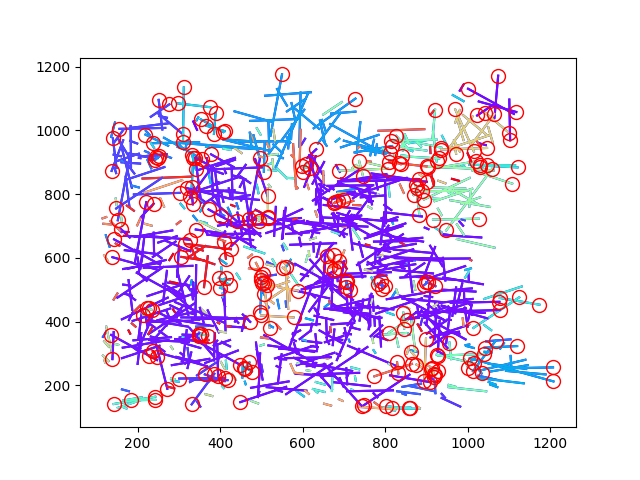
\includegraphics[width=0.7\linewidth]{3}
	\end{center}
	
	
	\vfill
	\newpage
	
	\section{Introducción}
	En esta práctica se nos propone encontrar las componentes conexas de un sistema de segmentos en el plano bidimensional. En concreto, los segmentos representan carriles de circulación, y el sistema es el mapa de una ciudad. 
	
	Si dos carriles se intersecan, entonces forman parte del mismo subsistema conexo de circulación, y sus transeúntes pueden llegar a todos sus puntos sin salirse de los carriles.
	
	Nuestro objetivo es contar cuántos subsistemas conexos hay, es decir, cuántas componentes conexas tiene el sistema.	
	
	\section{Material usado y metodología}
	Contamos con un sistema $A$ de 1000 segmentos aleatorios que nos vienen dados de antemano. Sus coordenadas oscilan entre 110 y 1230. Son, por tanto, un subespacio del plano $\mathbb{R}^2$.
	
	\subsection{Apartado \textit{i})}
	En el primer apartado, vamos a crear un algoritmo para calcular el número de componentes conexas de $N$ segmentos.
	
	Para ello, vamos a hacer uso de la conocida estructura de datos de conjuntos disjuntos, y del algoritmo Union-Find. Consiste en un conjunto de árboles, es decir, un bosque, y cada árbol se corresponde con un conjunto disjunto distinto. La raíz de cada árbol es el representante canónico del conjunto. 
	
	Si tenemos dos elementos que están en el mismo conjunto, se unen con la operación Union. Si queremos saber a qué conjunto pertenece un elemento, la operación Find devuelve la raíz de su árbol.
	
	Si la operación Union se implementa de la forma más ingenua, que es, por ejemplo, haciendo un nodo padre del otro, en el peor caso cada operación tarda un tiempo de $\mathcal{O}(n\log n)$ con $n$ el número de nodos. Si siempre se añade el árbol más pequeño al más grande, se mejora a $\mathcal{O}(\log n)$. 
	
	Sin embargo, este tiempo se puede reducir aún más, a $\mathcal{O}(\alpha(n))$, donde $\alpha(n)$ es la inversa de la función de Ackermann, que es, a todos los efectos prácticos, constante \textemdash es menor que 5 para todos los valores utilizables de $n$. Se consigue mediante la compresión del árbol cada vez que se busca un nodo: todos los nodos por el camino se ponen como hijos de la raíz para que siempre estén cerca.
	
	Gracias a este algoritmo, solo basta con encontrar las intersecciones de todos los segmentos, unirlos dentro de esta estructura, y contar cuántos árboles quedan.
	
	Para encontrar las intersecciones de todos los segmentos, podemos utilizar la forma más ingenua, que es comparar todos los pares en tiempo $\mathcal{O}(n^2)$. 
	
	También podemos utilizar el conocido algoritmo Sweep-Line. Consiste en escanear todos los puntos en orden de sus abscisas, y comprobar si los puntos iniciales acaban cruzándose con otros segmentos en un orden distinto a los iniciales. Es del orden de $\mathcal{O}(n\log n)$, y se pueden encontrar más detalles en mi trabajo \url{https://github.com/celrm/geometria-computacional/blob/master/files/main.pdf}.
	
	\subsection{Apartado \textit{ii})}
	En el segundo apartado representaremos el espacio $A$ y calcularemos con el algoritmo previo cuántas componentes conexas tiene (\texttt{n\_comp}).
	
	Para conseguir conectar todas las componentes, está claro que harían falta como máximo $\texttt{n\_comp}^2$ segmentos adicionales, que conectarían cada subsistema a pares. Sin embargo, esta cota se puede rebajar teniendo en cuenta las componentes colineales entre sí. De hecho, tres componentes son colineales si y solo si sus envolventes conexas lo son.
	
	\section{Resultados y conclusiones}
	\subsection{Apartado \textit{i})}
	El algoritmo que calcula las componentes conexas de un sistema de puntos $xy=(X,Y)$ se encuentra programado en la función \texttt{connected\_components}. Devuelve el número de componentes, el árbol Union-Find que relaciona cada índice de segmento con su índice representante, y la lista de segmentos. 
	
	Se ha implementado la manera cuadrática de calcular todas las intersecciones, pero también podría implementarse la forma más eficiente, en la función \texttt{find\_intersections}.
	
	\subsection{Apartado \textit{ii})}
	A continuación, se muestra el espacio $A$ de segmentos sobre el plano. Están coloreados en función de la componente conexa a la que pertenecen (aunque los colores no son únicos). 
	
\begin{center}
		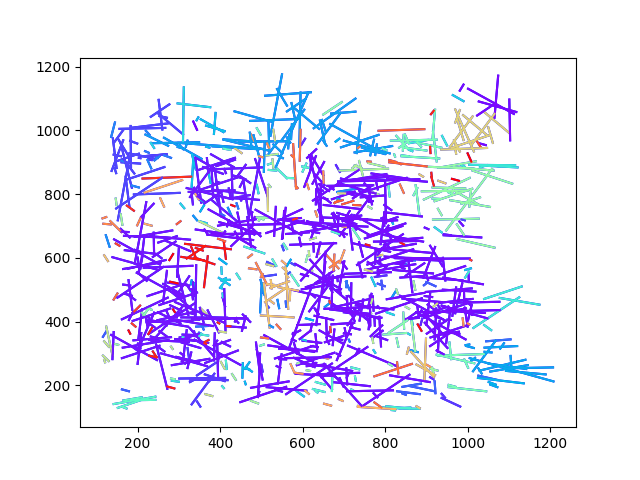
\includegraphics[width=0.7\linewidth]{2}
\end{center}
	
	El número de componentes conexas que devuelve el algoritmo es 338.
	
	Con este algoritmo podremos, de manera general, calcular el número de componentes conexas de cualquier sistema de segmentos en el plano arbitrario que nos propongan, y en un tiempo muy eficiente.
	
	
	\newpage
	\section{Código}\label{codigo}
	
	\lstinputlisting[language=Python]{Ejer3_GCOM2022-plantilla_conexas.py}
	
\end{document}
